% Prof. Dr. Ausberto S. Castro Vera
% UENF - CCT - LCMAT - Curso de Ci\^{e}ncia da Computa\c{c}\~{a}o
% Campos, RJ,  2023 
% Disciplina: An\'{a}lise e Projeto de Sistemas
% Aluno: 

\chapterimage{analise.png} % Table of contents heading image
\chapter{Etapa de An\'{a}lise}

Neste capítulo serão especificados e descritos os principais requisitos necessários para o funcionamento adequado do sistema computacional apresentado.



\section{Requisitos do Sistema}
\subsection{Hardware}
\begin{enumerate}
	\item Computadores
	\item Equipamentos de Rastreamento (GPS)
	\item Rede de Servidores
	\item Rede de Computadores
	\item Sensores de Monitoramento
	\item Câmeras de Segurança
	\item Equipamentos de Comunicação
	\item Tablets
	\item Smartphones
	\item Equipamentos de Gerenciamento de Rede
	\item Acesso a Rede
	\item Mobília
	\item Veículos da Frota
	\item Sistema de Ventilação
	\item Saídas de Emergência
	
	\subsection{Software}
	\item Softwares de Segurança (AntiVírus)
	\item Sistema de Cadastro de Usuários
	\item Sistema de Cadastro de Funcionários
	\item Firewalls
	\item Página Web Para Acesso de Usuários
	\item Sistema de Detecção de Invasões
	\item Sistema de Monitoramento da Carga
	\item Sistema de Rastreamento da Carga
	\item Interface Para Visualização de Informações da Carga
	\item Software de Filtragem de Conteúdo 
	\item Interface de Visualização e Gestão da Frota
	\item Sistema de Alerta de Problemas
	\item Sistema de Análise de Dados
	\item Editores de Documentos
	\item Sistema de Funcionários
	
	\subsection{Pessoas}
	\item Motoristas
	\item Programadores
	\item Gerente de Projeto
	\item Analista de Sistemas
	\item Pessoal de Monitoramento 
	\item Engenheiro de Software
	\item Pessoal de Logística
	\item Equipe de Manutenção
	\item Equipe de Segurança
	\item Analistas de Dados
	\item Equipe de Limpeza
	\item Equipe de TI
	\item Secretários(as)
	\item Equipe de Atendimento ao Cliente
	
	\subsection{Banco de Dados e Nuvem}
	\item Segurança de BD's
	\item Servidor Dedicado
	\item Segurança dos Servidores
	\item Backup Semanal
	\item Armazenamento de Logs
	\item Backup de Dados Local
	\item Backup de Dados em Nuvem
	\item Registro de Dados dos Funcionários
	\item Registro de Dados dos Usuários
	\item Registro de Dados das Entregas
	\item Confiabilidade de Dados
	\item Registro de Rotas
	\item Registro do Trânsito das Rotas
	
	\subsection{Documentos}
	\item Manual do Sistema
	\item Documentação de Treinamento 
	\item Relatórios Semanais
	\item Editor de Documentos
	\item Salvar Documentos
	\item Impressão de Relatórios
	\item Termos e Contratos
	\item Orçamentos
	
	\subsection{Metodologias e Procedimentos}
	\item Treinamento de Funcionários
	\item Gerenciamento do Sistema
	\item Metodologia de Desenvolvimento Adequada
	\item Gerenciamento de Recursos
	\item Planejamento do Desenvolvimento
	\item Bateria de Testes
	\item Procedimentos de Implementação
	\item Protocolos de Segurança
	\item Modelagem do Sistema
	
	\subsection{Mobilidade}
	\item Computadores
	\item Notebooks
	\item Tablets
	\item Smartphones
	\item Televisores
	\item Roteadores de Internet
	\item Serviços de Dados Móveis
	\item Sistema de Rastreamento
\end{enumerate}

\section{Definição de Requisitos}
\begin{enumerate}
	\item \textbf{Computadores}: O sistema deve possuir computadores de ótima qualidade para o gerenciamento e utilização do sistema.
	
	\item \textbf{Equipamentos de Rastreamento(GPS)}: O sistema deve apresentar equipamentos de rastreamento nos veículos.
	
	\item \textbf{Rede de Servidores}: O sistema deve possuir uma ótima rede de servidores para armazenamento de dados
	
	\item \textbf{Rede de Computadores}: O sistema deve ter uma boa instalação e manutenção de redes ao alcance dos computadores.
	
	\item \textbf{Sensores de Monitoramento}: O sistema deve possuir um gama de sensores para monitoramento da carga.
	
	\item \textbf{Câmeras de Segurança}: O sistema deve possuir câmeras de segurança para monitoramento da carga.
	
	\item \textbf{Tablets ou Smartphones}: O sistema deve possuir Tablests ou Smartphones de qualidade, que permitem a comunicação entre motoristas e equipe.
	
	\item \textbf{Acesso a Rede}: O sistema deve possuir acesso a uma rede de internet de qualidade, permitindo a ideal utilização do sistema.
	
	\item \textbf{Software de Segurança}: O sistema deve apresentar Softwares de segurança que assegurem a utilização do sistema e computadores, evitando invasões.
	
	\item \textbf{Sistema de Cadastro de Usuários}: O sistema deve apresentar um sistema de cadastro de usuários adequado para o acesso de usuários ao sistema.
	
	\item \textbf{Página Web Para Acesso de Usuários}: O sistema deve possuir uma página web com interface amigável dedicada ao acesso do usuário.
	
	\item \textbf{Sistema de Análise de Dados}: O sistema deve possuir um sistema que possibilite a análise e processamento dos dados adquiridos.
	
	\item \textbf{Motoristas}: O sistema deve possuir uma equipe de motoristas responsável por dirigir os veículos e realizar as entregas.
	
	\item \textbf{Registro de Dados de Usuários}: O sistema deve apresentar um armazenamento seguro e confiável de dados necessários dos usuários.
	
	\item \textbf{Manual do Sistema}: O sistema deve possuir um manual responsável por descrever o funcionamento do sistema.
	
	\item \textbf{Treinamento de Funcionários}: O sistema deve realizar treinamentos com funcionários para o uso adequado do sistema.
\end{enumerate}

\section{Especificação de Requisitos}
\begin{itemize}
	\item \textbf{Cadastro de Funcionários} \begin{enumerate}
		\item Cadastro do username, senha e dados
		\item Cadastro dos dados no banco de dados
		\item Validação dos dados de login
		\item Permitir a entrada
	\end{enumerate}

	\item \textbf{Página Web Para Acesso de Usuários} \begin{enumerate}
		\item Criação da página
		\item Formatação de interface amigável
		\item Área de login
		\item Possibilidade de ver os dados
	\end{enumerate}

	\item \textbf{Sistema de Rastreamento da Carga} \begin{enumerate}
		\item Cadastro do funcionário no sistema
		\item Cadastro dos dados no banco de dados
		\item Validação do login
		\item Exibição dos dados 
	\end{enumerate}

	\item \textbf{Programadores} \begin{enumerate}
		\item Busca por funcionários
		\item Processo de entrevista de emprego
		\item Selecionamento de candidatos
		\item Capacitação/treinamento da equipe de funcionários
		\item Testes da equipe
	\end{enumerate}

	\item \textbf{Bateria de Testes} \begin{enumerate}
		\item Desenvolvimento do sistema até a etapa de testes
		\item Idealização da bateria de testes pela equipe de teste
		\item Implementação da bateria de testes
		\item Verificar resultados e consertar possíveis erros
	\end{enumerate}

	\item \textbf{Confiabilidade de Dados} \begin{enumerate}
		\item Desenvolvimento dos termos de uso de dados do usuário
		\item Sistema de segurança dos bancos de dados eficiente
		\item Uso ético dos dados do usuário 
	\end{enumerate}

	\item \textbf{Backup Semanal} \begin{enumerate}
		\item Definição de data e hora para backup
		\item Padronização de formato do backup
		\item Realização do Backup de maneira segura e confiável
	\end{enumerate}

	\item \textbf{Equipamentos de Rastreamento (GPS)} \begin{enumerate}
			\item Compra de equipamentos de qualidade e adequados
			\item Instalação dos equipamentos nos veículos
			\item Conexão dos equipamentos com o sistema
			\item Calibração dos equipamentos e execução de teste
			\item Treinamento de funcionários para a utilização dos mesmos
		\end{enumerate}
\end{itemize}	

\section{Stakeholders}
Stackholders: 
\begin{itemize}
	\item \textbf{Clientes:} Destinatários das entregas.
	\item \textbf{Equipe de Logística:} Responsáveis pela gerência das operações de entregas.
	\item \textbf{Motoristas:} Responsáveis pela realização das entregas.
	\item \textbf{Gerente de Frota:} Responsável por gerenciar a frota de veículos.
	\item \textbf{Equipe de Atendimento:} Responsáveis por prestar suporte ao cliente.
	\item \textbf{Departamento de TI:} Responsáveis por manter e aprimorar o funcionamento do sistema.
	\item \textbf{Fornecedores de Tecnologia:} Responsáveis por fornecer a tecnologia utilizada pelo sistema para que tenha seu funcionamento adequado.
	\item \textbf{Gerente de Vendas e Marketing:} Responsável por promover o serviço prestado.
	\item \textbf{Acionistas e Investidores:} Responsáveis por manter a saúde financeira do sistema estável.
	\item \textbf{Reguladores e Autoridades:} Responsáveis por monitorar se o sistema atua corretamente vigente as leis.                  
\end{itemize}

Pontos de vista: 
\begin{itemize}
	\item \textbf{Ponto de Vista do Cliente:} Concentra no ponto de vista da relação do cliente com o sistema, trazendo uma melhor experiência e confiabilidade do mesmo em relação a sua entrega.
	
	\item \textbf{Ponto de Vista do Motorista:} Concentra na relação entre o motorista responsável pela entrega com o sistema, trazendo uma melhor interação entre o mesmo e a central, otimizando o processo de entrega e resolução de possíveis problemas.
	
	\item \textbf{Ponto de Vista da Equipe:} Concentra a relação entre a equipe e a frota, possibilitando uma análise adequada dos dados e resolução de possíveis problemas durante as viagens.
	
	\item \textbf{Ponto de Vista dos Proprietários e Investidores:} Concentra no interesse dos proprietários e investidores no retorno financeiro da empresa.
\end{itemize}

\section{Entrevista}
A etapa de entrevista é extremamente importante para a criação e modelagem do sistema, visto que por meio dela é possível ter contato direto com os stackholders do sistema afim de recolher informações uteis com o intuito de moldar os requisitos do sistema com base em respostas dadas pelo mesmo para uma sequência de perguntas. A seguir será apresentado um possível cenário de uma entrevista com um dos membros da equipe de logística do sistema sobre dificuldades enfrentadas em um sistema antigo, e expectativas sobre a implementação do sistema D.S.S.

\textbf{Entrevistador:} Quais são as principais metas que deseja alcançar com a implementação do sistema D.S.S?

\textbf{Entrevistado:} Nossas metas são: alcançar a uma maior eficiência das entregas, a redução dos custos totais, melhora na segurança da carga e maior satisfação do cliente.

\textbf{Entrevistador:} Como o sistema atual prejudica nesse cenário?

\textbf{Entrevistado:} O sistema usado atualmente dificulta a eficiência das entregas porque não é possível obtermos dados precisos das rotas, como o trânsito, instabilidades que possam ocorrer na área e outras dificuldades do percurso, o que eleva o tempo gasto nas entregas, e por consequência os custos de viagem. Além disso, não existe nenhum recurso atualmente que nos permita garantir a segurança da carga transportada.

\textbf{Entrevistador:} Quais melhorias seriam necessárias para serem implementadas no sistema D.S.S?

\textbf{Entrevistado:} As principais melhorias que esperamos serem implementadas são: maior precisão do rastreamento da carga, maior número informações de todo o percurso da entrega, melhor interação entre frota e central.

\textbf{Entrevistador:} Você acha necessário a implementação dessas melhorias?

\textbf{Entrevistado:} Sim, visto que com a implementação dessas melhorias é possível realizar uma otimização do tempo de entrega e por consequência uma redução significativa dos custos operacionais, além disso a segurança seria extremamente melhorada.

\section{ Casos de Uso}

Nessa seção serão abordados alguns dos principais casos de uso do sistema D.S.S.

\subsection{Rastreamento de Entregas}
Permite o usuário obter a localização da entrega em tempo real.
\begin{enumerate}
	\item Usuário acessa o sistema
	\item Usuário faz o login
	\item Usuário seleciona o produto desejado
	\item Usuário obtém informações relevantes da entrega inclusive a localização atual
	\item Sair do sistema
\end{enumerate}

\subsection{Planejamento de Rotas}
Permite a equipe especializada planejar as rotas da frota de maneira mais eficiente possível.

\begin{enumerate}
	\item Usuário acessa o sistema
	\item Usuário efetua o login
	\item Usuário obtém acesso ao Status de inúmeras entregas em andamento e antigas 
	\item Usuário seleciona a entrega desejada
	\item Usuário recebe uma sequência de dados pertinentes sobre a entrega
	\item Usuário realiza uma análise das informações recolhidas
	\item Usuário produz relatórios e chega a conclusões
	\item Sair do sistema
\end{enumerate}

\subsection{Gerenciamento da Frota}
Permite a equipe especializada gerenciar a frota de veículos de forma adequada.
\begin{enumerate}
	\item Usuário acessa o sistema
	\item Usuário efetua o login
	\item Usuário obtém acesso ao Status de inúmeros veículos da frota
	\item Usuário seleciona o veículo desejado
	\item Usuário realiza as ações desejadas (se comunicar com o motorista, analisar dados, propor mudanças de rota e etc)
	\item Sair do sistema
\end{enumerate}

\subsection{Diagrama de Casos de Uso}
Essa seção apresentará uma representação gráfica de um diagrama de casos de uso que serve para descrever as interações entre um sistema e seus atores.

\begin{figure}[H]
	\centering
	\includegraphics[width=1\linewidth]{"Pictures/Diagrama Casos de Uso"}
	\caption{}
	\label{fig:diagrama-casos-de-uso}
\end{figure}
\section{Modelagem}
    \subsection{Diagrama de Fluxo de Dados}
	O diagrama de fluxo de dados é uma forma gráfica de representar a forma de como os dados são processados, armazenados e movidos em um respectivo sistema.
	
	O diagrama abaixo representa um diagrama de fluxo de dados da etapa de login de um usuário ao sistema.
% TODO: \usepackage{graphicx} required
\begin{figure}[H]
	\centering
	\includegraphics[width=1\linewidth]{"Pictures/Fluxo de Dados Login"}
	\caption{}
	\label{fig:fluxo-de-dados-login}
\end{figure}

	O diagrama abaixo representa um diagrama de fluxo de dados da acesso de um cliente ao sistema, mostrando informações desejadas de sua respectiva entrega, assim como a possibilidade de entrar em contato com um suporte.
% TODO: \usepackage{graphicx} required
\begin{figure}[H]
	\centering
	\includegraphics[width=1\linewidth]{"Pictures/Fluxo de Dados1"}
	\caption{}
	\label{fig:fluxo-de-dados1}
\end{figure}

	O diagrama abaixo representa a etapa de acesso ao sistema por parte da equipe de logística da empresa.
% TODO: \usepackage{graphicx} required
\begin{figure}[H]
	\centering
	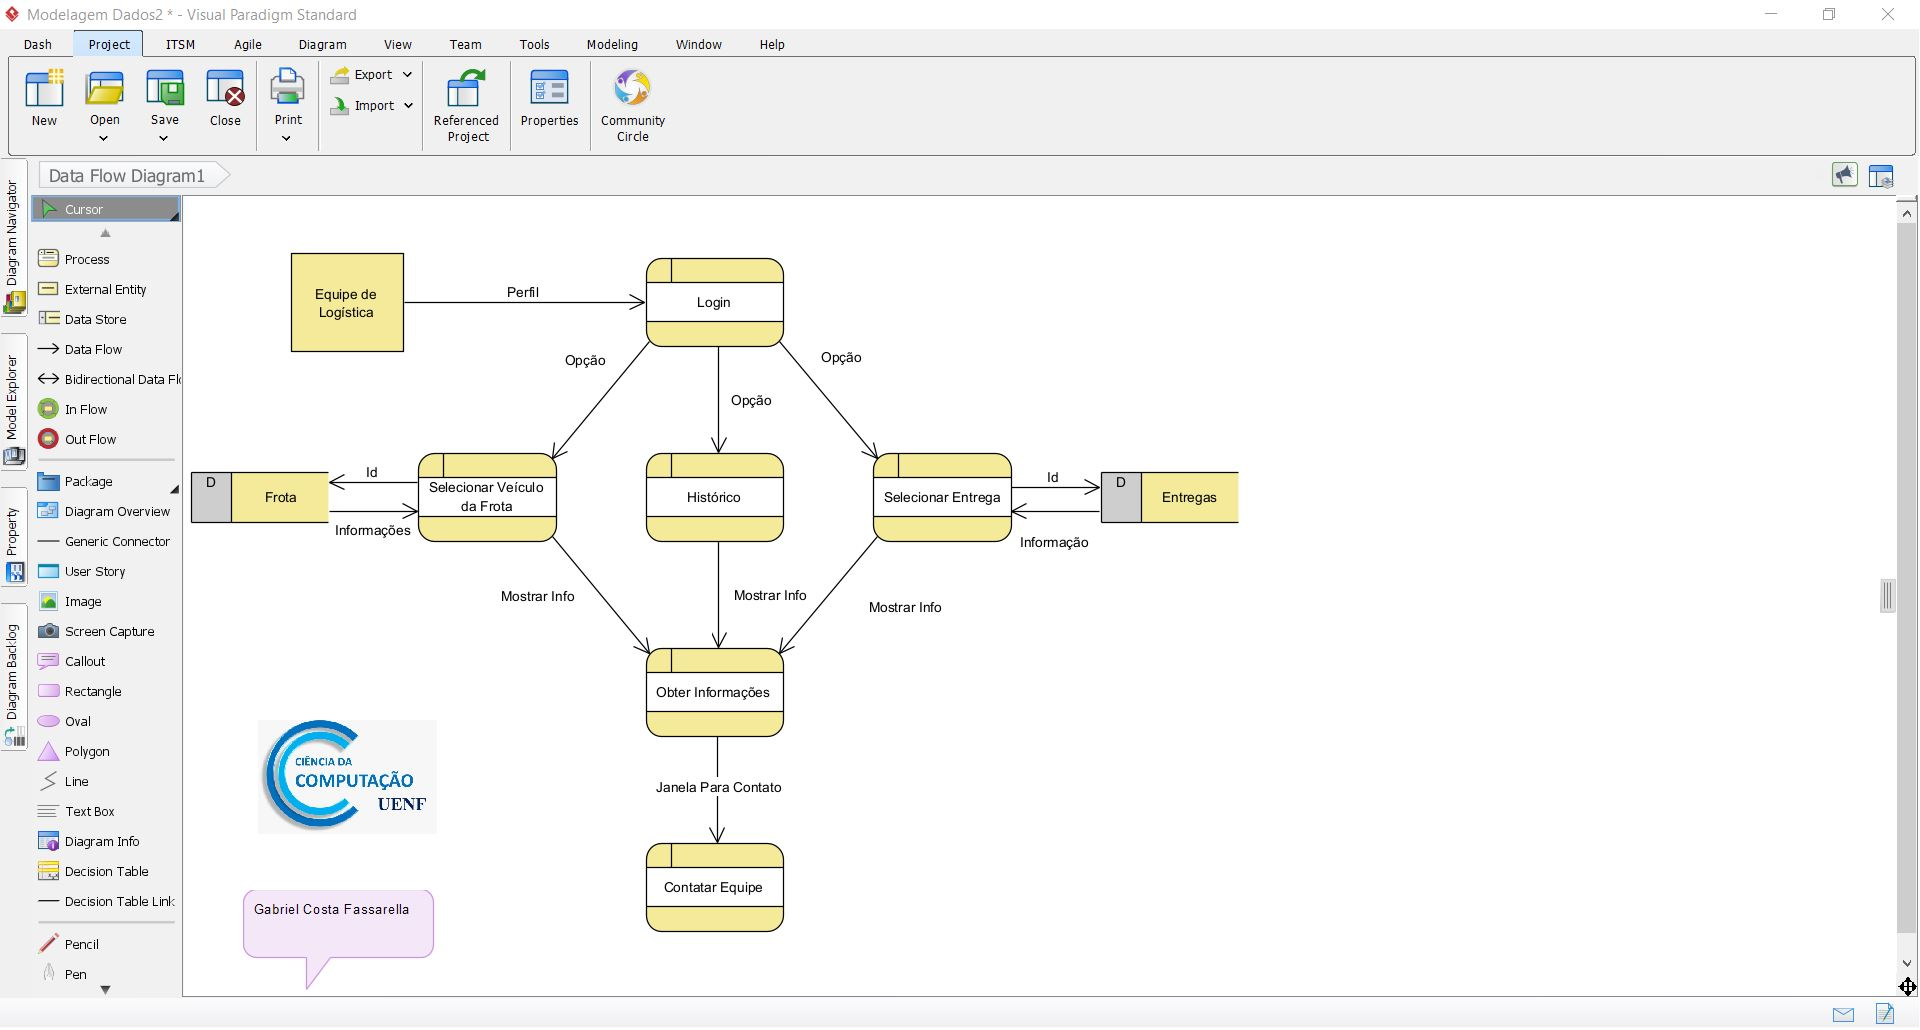
\includegraphics[width=1\linewidth]{Pictures/Flux2}
	\caption{}
	\label{fig:flux2}
\end{figure}

    \subsection{Diagrama de Entidades e Relacionamentos}
	Um Diagrama de Entidade-Relacionamento (ER) é uma representação gráfica que descreve as entidades (objetos ou conceitos) e os relacionamentos entre eles em um sistema. Os diagramas ER ajudam a visualizar a estrutura de um sistema, identificando as principais entidades e como elas se relacionam.
	
	% TODO: \usepackage{graphicx} required
	\begin{figure}[H]
		\centering
		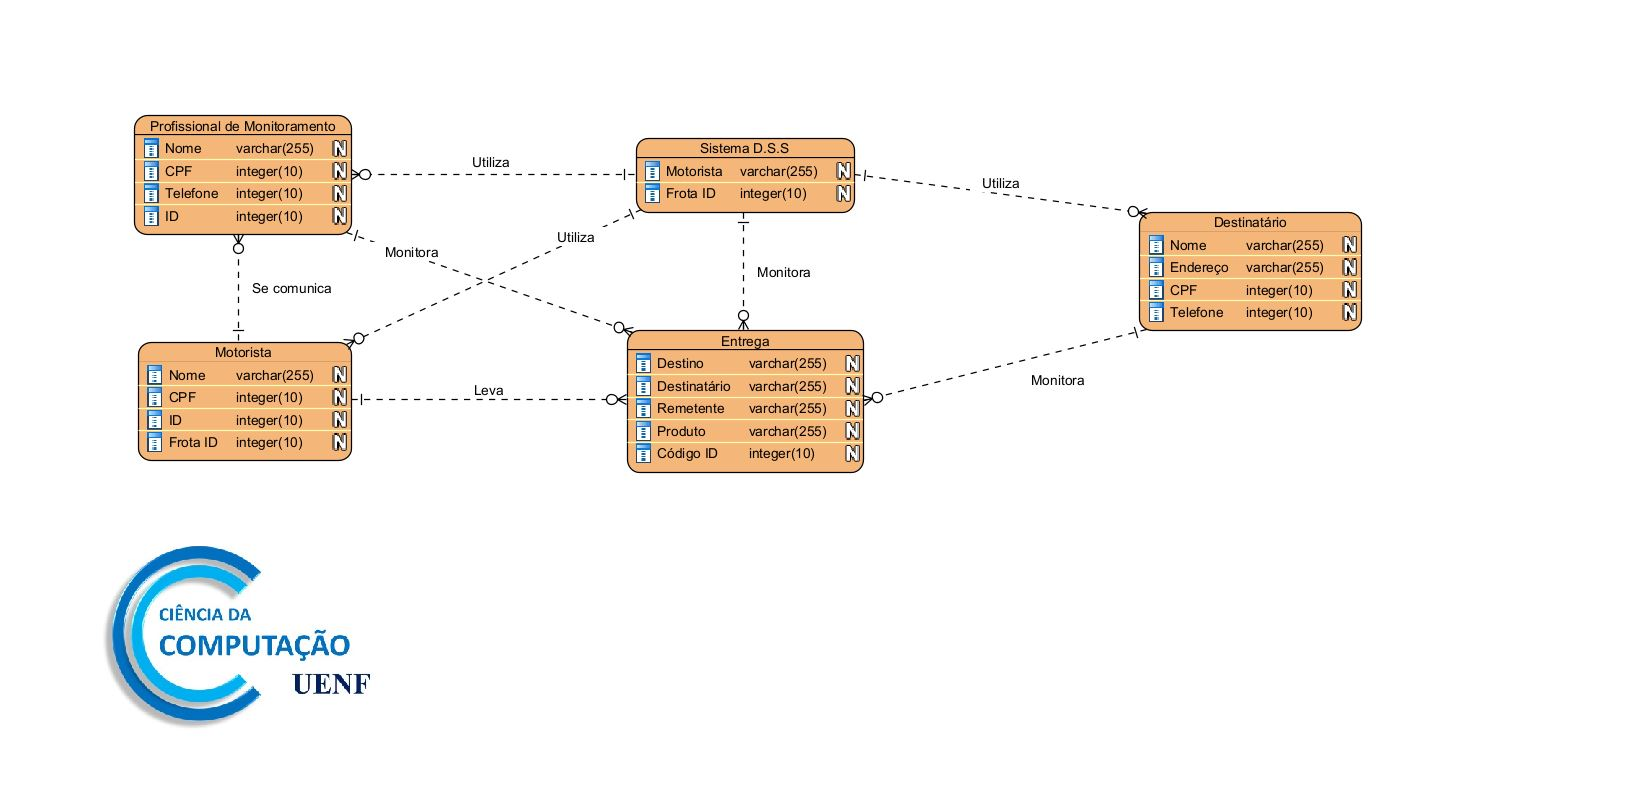
\includegraphics[width=1.2\linewidth]{Pictures/ER1}
		\caption{}
		\label{fig:er1}
	\end{figure}

	
	% TODO: \usepackage{graphicx} required
	\begin{figure}[H]
		\centering
		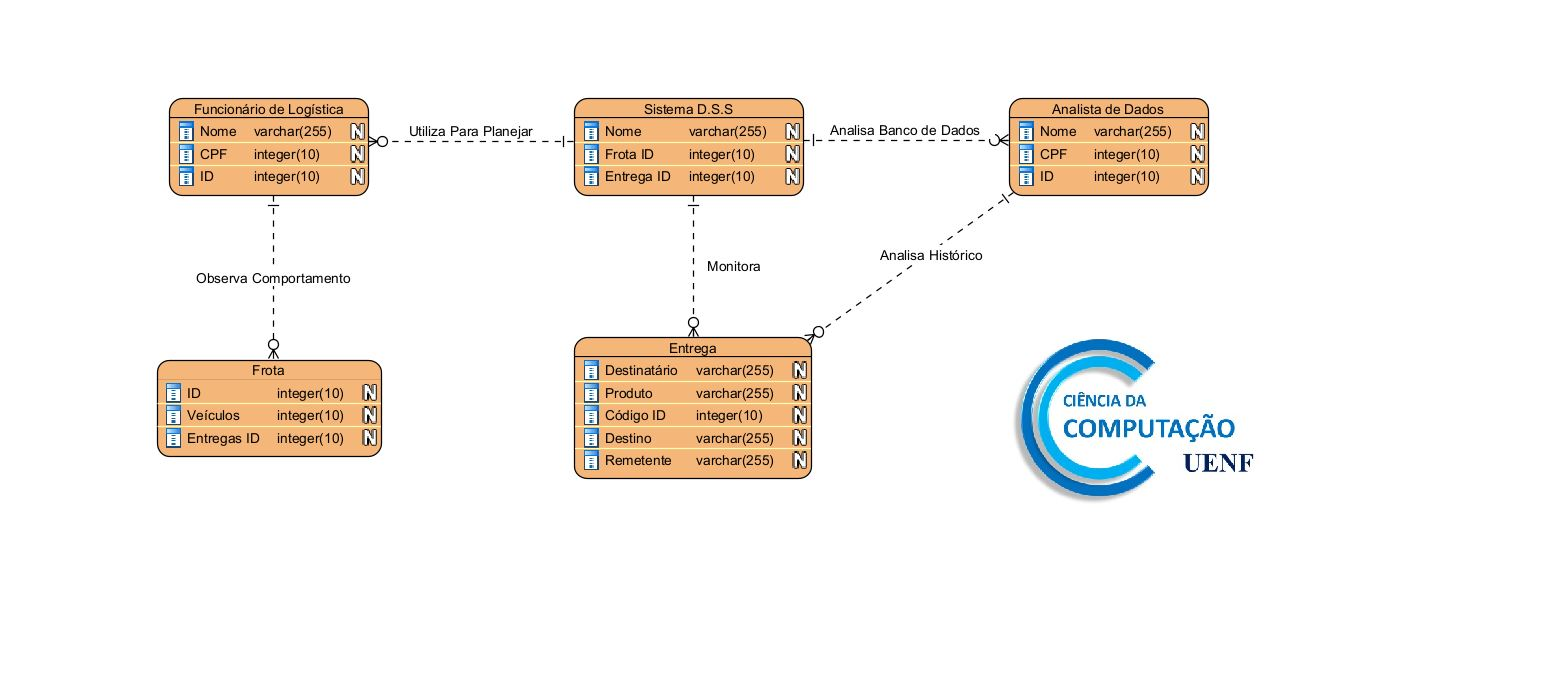
\includegraphics[width=1.2\linewidth]{Pictures/ER2}
		\caption{}
		\label{fig:er2}
	\end{figure}

